\documentclass[TechnicalNoteMeteo.tex]{subfiles}

\begin{document}

\subsection{Materials and Method}

\subsubsection{Study Area}

The algorithm was tested using data from 32 land-based Canadian weather stations in and around the Monteregie Est region, located in southern Quebec, Canada. This region covers a total area of \SI{9032}{km^2}, from the St. Lawrence River at its northern limit to the border of the United States (states of New York and Vermont) at its southern limit (see Figure X). It is characterized by strongly variable topography and land cover conditions. The climate of this region is characterized by significant seasonal differences in temperature, resulting in warm summers and cold winters. Total precipitation, as rain or snow, are distributed rather evenly throughout the year.

\subsubsection{Weather Dataset}

A total of 32 weather stations were selected from the Canadian Daily Climate Database (CDCD) based on the availability and continuity of the measured weather data between 1980 and 2014. \Cref{tab:selectedStations} presents the list of these selected stations with their corresponding climate~ID, location coordinates (latitude and longitude), altitude, time periods for which data were available, yearly averages and percentage of days with missing data. Most of the information presented in \cref{tab:selectedStations} are generated automatically when loading data into the gap-filling routine and saved in a file named `weather\_datasets\_summary.log' within the previously defined output folder. The geographical disposition of the weather stations is also presented in the map of \cref{fig:Thiessen_meteo}.

The data were downloaded and formatted to the format described in \cref{subsec:input} using the software WHAT \citep{gosselin_user_2015}. WHAT provides a graphical interface to the online CDCD that allows to search for stations interactively using location coordinates, download the available data for the selected weather stations, and automatically organize the data in a format that is compatible with the gap-filling algorithm presented in this paper.

\begin{table}[!p]
    \centering
    \setstretch{1.25}
    \caption{List of selected weather stations in the study area and related information about missing data for the 1980-2014 period}
    \rowcolors{6}{gray!10}{}
    \resizebox{1.\linewidth}{!}{
    \begin{tabular}{            
        S[table-format = 2]
        l
        *2S[table-format = 2.2]
        S[table-format = 3.1]
        *4S[table-format = 2.1]
        S[table-format = 2.1]
        S[table-format = -1.1]
        S[table-format = 1.1]
        S[table-format = 4.1]
    	}
    	\toprule
    	\multicolumn{5}{c}{} & \multicolumn{4}{c}{\% of days with missing data} & \multicolumn{4}{c}{Yearly Averages}\\
    	\cmidrule(lr){6-9}
    	\cmidrule(lr){10-13}
    	{\#} & {Station} & {Lat.} & {Lon.} & {Alt.} & {T\textsubscript{max}} & {T\textsubscript{min}} & {T\textsubscript{mean}} & {P\textsubscript{tot}} & {T\textsubscript{max}} & {T\textsubscript{min}} & {T\textsubscript{mean}} & {P\textsubscript{tot}} \\
    	& {name} & {\SIUnitSymbolDegree N} & {\SIUnitSymbolDegree W} & {m} & {\%} & {\%} & {\%} & {\%} & {\SIUnitSymbolCelsius} & {\SIUnitSymbolCelsius} & {\SIUnitSymbolCelsius} & {mm} \\
    	\midrule
        1 & Auteuil & 45.65 & 73.73 & 53.0 & 20.8 & 19.1 & 22.8 & 18.4 & 11.3 & 1.4 & 6.4 & 989.7 \\
        2 & Bonsecours & 45.40 & 72.27 & 297.2 & 4.7 & 5.1 & 6.3 & 3.2 & 10.0 & -0.8 & 4.6 & 1226.2 \\
        3 & Brome & 45.18 & 72.57 &  205.7 & 2.6 & 2.3 & 3.0 & 2.3 & 11.0 & -0.4 & 5.3 & 1296.7 \\
        4 & Bromptonville & 45.48 &  71.95 &  130.0 & 3.9 & 4.2 & 6.0 & 1.8 & 11.1 & -0.1 & 5.5 & 1137.9 \\
        5 & Danville & 45.82 & 71.98 & 190.0 & 30.8 & 31.1 & 33.1& 30.2 & 10.6 & 0.4 & 5.5 & 1074.5 \\
        6 & Drummondville & 45.88 & 72.48 & 82.3 & 2.5 & 2.4 & 3.4 & 1.8 & 11.0 & 1.5 & 6.2 & 1122.1 \\
        7 & Farnham & 45.30 & 72.90 & 68.0 & 5.2 & 4.7 & 6.1 & 3.7 \\
        8 & Fleury & 45.80 & 73.00 & 30.5 & 1.1 & 1.2 & 1.6 & 1.1 \\
        9 & Georgeville & 45.13 & 72.23 & 266.7 & 26.5 & 26.2 & 27.6 & 5.7 \\
        10 & Granby & 45.38 & 72.72 & 175.0 & 1.3 & 1.3 & 2.1 & 0.5 \\
        11 & Hemmingford & 45.07 & 73.72 & 61.0 & 6.0 & 6.0 & 6.8 & 4.6 \\
        12 & Iberville & 45.33 & 73.25 & 30.5 & 7.3 & 7.5 & 9.7 & 4.2 \\
        13 & Magog & 45.27 & 72.12 & 274.0 & 4.2 & 4.2 & 5.3 & 4.6 \\
        14 & Marieville & 45.40 & 73.13 & 38.0 & 10.2 & 10.4 & 11.2 & 9.8 \\
        15 & Nicolet & 46.20 & 72.62 & 30.4 & 4.1 & 4.2 & 5.2 & 3.6 \\
        16 & Philipsburg & 45.03 & 73.08 & 53.3 & 4.9 & 5.1 & 6.9 & 3.2 \\
        17 & Pierreville & 46.08 & 72.83 & 15.2 & 6.3 & 5.4 & 6.9 & 4.9 \\
        18 & Richmond  & 45.63 & 72.13 & 123.1 & 3.3 & 3.3 & 3.8 & 4.0 \\
        19 & Riviere des Prairies & 45.70 & 73.50 & 9.0 & 2.4 & 4.0 & 4.8 & 1.4 \\
        20 & Sabrevois & 45.22 & 73.20 & 38.1 & 25.5 & 26.0 & 27.1 & 5.2 \\
        21 & Sorel & 46.03 & 73.12 & 14.6 & 5.7 & 5.9 & 6.2 & 4.5 \\
        22 & St. Amable & 45.67 & 73.30 & 41.1 & 8.6 & 10.4 & 11.8 & 7.7 \\
        23 & St. Bernard & 45.08 & 73.38 & 49.3 & 9.6 & 9.7 & 10.5 & 9.0 \\
        24 & St. Guillaume & 45.88 & 72.77 & 43.9 & 4.3 & 4.6 & 5.7 & 3.0 \\
        25 & St.Hyacinthe 2 & 45.57 & 72.92 & 33.0 & 6.7 & 6.9 & 7.5 & 6.6 \\
        26 & St. Jacques & 45.95 & 73.58 & 69.0 & 11.7 & 11.9 & 14.0 & 10.8 \\
        27 & St. Janvier & 45.73 & 73.88 & 61.0 & 40.5 & 40.7 & 41.6 & 21.9 \\
        28 & St. Nazaire & 45.73 & 72.62 & 68.6 & 3.8 & 3.8 & 5.4 & 2.7 \\
        29 & Ste. Madeleine & 45.62 & 73.13 & 30.0 & 5.8 & 6.4 & 7.0 & 5.1 \\
        30 & Ste. Martine & 45.22 & 73.85 & 38.1 & 6.9 & 6.6 & 7.8 & 6.4 \\
        31 & Sutton & 45.07 & 72.68 & 243.8 & 0.4 & 0.6 & 0.7 & 0.5 \\
        32 & Vercheres & 45.77 & 73.37 & 21.0 & 3.5 & 3.5 & 4.7 & 2.2 \\
        \bottomrule
    \end{tabular}
    }
    \label{tab:selectedStations}
\end{table}

Total annual precipitation for all of these stations, the mean annual precipitation is \SI{1100}{mm/y}. The highest total precipitation are observed at the Brome station ($\sim$\SI{1280}{mm/y}), while the lowest at the Sorel station ($\sim$\SI{960}{mm/year}). Mean annual air temperature in the study area is \SI{5.9}{\celsius}, ranging from \SIrange{4.3}{6.7}{\celsius} while average monthly temperatures fluctuate between \SIrange{-12}{21}{\celsius}. The minimum monthly temperatures are observed in January \SIrange{-17.1}{-13.6}{\celsius}) while the maximum monthly temperatures are observed in July (\SIrange{24}{26.7}{\celsius}).
The highest temperatures are observed at the Philipsburg et Saint-Bernard stations and the lowest at Bonsecours station.

\begin{figure}
    \centering
    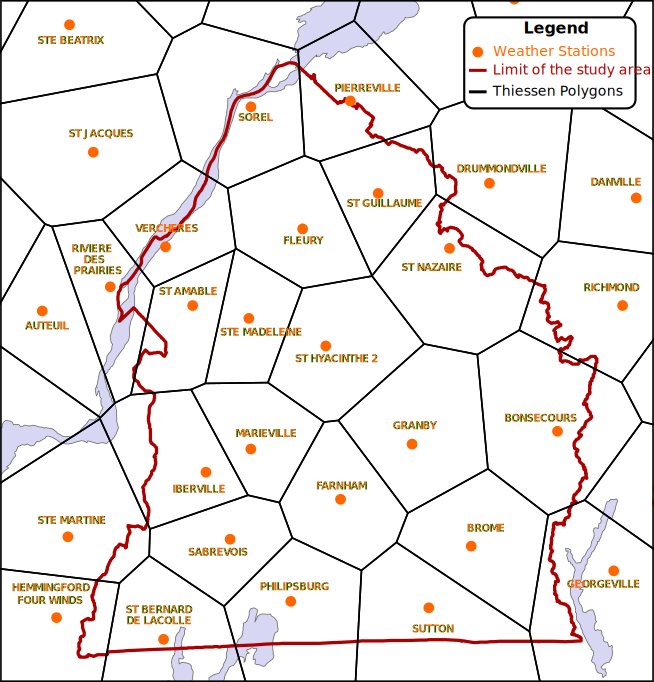
\includegraphics[width=0.5\textwidth]{img/Thiessen_meteo}
    \caption[Locations of the weather stations in the Monteregie Est area.]{Locations of the weather stations in the Monteregie Est area.}
    \label{fig:Thiessen_meteo}
\end{figure}

\subsubsection{Gap-Filling the Data}

Missing data were estimated for the weather station located inside the Monteregie Est regions. The method was tested with the parameter value that are set by default in the algorithm, as shown in \cref{tab:method_parameter}.

The missing weather data and fill the gaps in the weather dataset of the station located within the study area. Stations bordering the limits but outside the study area were used to fill the data of the stations within the area, but their data were not filled. Data from these stations were use only to improve the spatial distribution of the neighboring stations for the weather station in the study area located near the limits.

The default value for the method parameters were kept in the algorithm. That is, the maximum number of neighboring station was set to 4, the horizontal and vertical distance thresholds were kept at 100 and 350 values respectively. The data were filled using the OLR and LRM method to see if it makes any real difference. Also, during the entire process, the option for the cross-validation was activated.

The accuracy of the method was also assessed with different value imposed on the maximum number of neighboring stations to see the impact on the accuracy of the method.

\subsection{Results}

The quality of the estimates is strongly affected by seasonality. Stations at higher elevations are difficult to estimate accurately, in large part because of the topographical diversity of the surrounding stations leading to degradation of spatial coherence among stations.

The tendency for all of the methods to have a negative bias is indicative of the nature of precipitation distributions to be positively skewed (interpolated values will tend to cluster about the median error rather than the mean).

According to \cite{xia_forest_1999}, the two most important factors in climatology are the inter-correlations in the station network, and the seasonal variations in the relations between the stations.

\subsection{Discussion}

However, weighing and regression-based techniques, including the MLR method, all tend to overestimate the number of rainy days, while heavy precipitation events are systematically underestimated. Therefore, the rainfall probability distribution is usually not preserved with these techniques). However, Simolo et al. (2010) have proposed a two-step procedure to modify the MLR method to address these issues.

An alternative approach would have been to calculate the correlation coefficient with a subset of data from the target series centered around the missing value, as it was done in Simolo et al. (2010) for instance. This approach allows for a better representation of the seasonal variations in the relationships between the stations. The downsides include a more complex algorithm to implement and a reduction of the method robustness and efficiency.

\end{document}